\lysh{33587}{4}

\begin{alist}
\item Το τριώνυμο $f(x) = -x^2 + 2x + 3$ έχει διακρίνουσα $\Delta = 2^2 - 4 \cdot (-1) \cdot 3 = 4 + 12 = 16 > 0$. Το
άθροισμα των ριζών του είναι $S = x_1 + x_2 = \dfrac{-2}{-1} = 2$ και το γινόμενό τους είναι
$P = x_1 \cdot x_2 = \dfrac{3}{-1} = -3$. Άρα $x_1 = 3, x_2 = -1$ και το πρόσημο του τριωνύμου είναι

\begin{center}
\begin{tikzpicture}
\tikzset{t style/.style = {style = dashed}}
\tkzTabInit[color,lgt=3,espcl=2,colorC = maincolor!40,
colorL = maincolor!20,
colorV = maincolor!40]%
{$x$ / .8,$-x^2 +2 x +3$ /0.8}%
{$-\infty$,$-1$,$2$,$+\infty$}%
\tkzTabLine{ , $-$, z
, $+$ , z
, $-$ , }
\end{tikzpicture}
\end{center}

Οπότε το τριώνυμο παίρνει θετικές τιμές για $x \in (-1, 3)$ και αρνητικές τιμές για
$x \in (-\infty, -1) \cup (3, +\infty)$.

\item Εφόσον $2,999 \in (-1, 3)$, από τον παραπάνω πίνακα προσήμου θα είναι $f(2,999) > 0$ και
επειδή $-1,002 < -1$ θα είναι $f(-1,002) < 0$. Άρα,
$f(2,999) \cdot f(-1,002) < 0$.

\item Αν $-3 < \alpha < 3 \Leftrightarrow |\alpha| < 3$, δηλαδή $0 \le |\alpha| < 3$, τότε ο αριθμός
$-\alpha^2 + 2|\alpha| + 3 = -|\alpha|^2 + 2|\alpha| + 3 = f(|\alpha|)$ είναι θετικός, όπως προκύπτει από τον πίνακα
προσήμου του τριωνύμου $f(x) = -x^2 + 2x + 3$ στο $\alpha)$ ερώτημα.
\end{alist}

